\documentclass[10pt,letterpaper]{article}

\usepackage[
  letterpaper,
  left=0.8125in,
  right=0.8125in,
  top=1in,
  bottom=1.125in,
  columnsep=0.3125in
]{geometry}
\usepackage{times}
\usepackage{graphicx}
\usepackage{float}
\usepackage{amsmath}
\usepackage{amssymb}
\usepackage{booktabs}
\usepackage{microtype}
\usepackage{xurl}
\usepackage[section]{placeins}
\usepackage[breaklinks=true,bookmarks=false]{hyperref}

\usepackage[backend=biber,style=numeric,sorting=none]{biblatex}
\addbibresource{ComputerVision.bib}

\pagestyle{empty}
\setlength{\emergencystretch}{2em}

\title{A Depth-Aware, Physics-Based Data Augmentation Framework for Simulating Rain and Fog
Distortions in Outdoor-RGB Images}
\author{
Rongxuan Duan\\
Pioneer Research Institute\\
{\tt\small }
}
\date{}


\begin{document}

\twocolumn[
\begin{@twocolumnfalse}
\maketitle

\begin{abstract}
\end{abstract}

\vspace{1em}
\end{@twocolumnfalse}
]
\section{Introduction}
Images used in computer vision are often distored. Distortion in computer vision refers to any signal that produces visual deviation in image/video 
from its original expectation. When the original iamge/video is unavailable, an observed visual comfort or simply annoying effect
on the aesthetic visual appearance is also considered as a distortion~\cite{muhammadaliqureshiDistortionClassificationComputer}. These distortions could be
sorted as In-Capture Distortion, including blur, noise, uneven illumination, color shifts, haze,
rain, snow, and other visibility changes; and Post-Capture Distortion, such as transmission,
impairments, enhancement artefacts, and adversarial distortion. Although these effects may
appear minor to human observers, they can change the statistical structure of an image and reduce
the reliability of machine learning models trained primarily on clean
data~\cite{muhammadaliqureshiDistortionClassificationComputer}. Distortions affect the
performances of high-level tasks, such as object classification, object detection, and scene
understanding~\cite{muhammadaliqureshiDistortionClassificationComputer}. Therefore, distortion
detection and removal are a possible preprocessing step for high-level tasks to decrease the
impact on performance.

For machine learning, distortion is not only an image-quality issue but also is affected by dataset and
training. Models usually learn from the distribution of inputs they are given, so a model
trained only on clean images may have poor generalizability when working on the same object
appearing under poor visibility, weather effects, or degraded contrast. Distortion-specified
datasets are important because they make it possible to evaluate model robustness by type and severity, 
rather than reporting only a single clean-data accuracy score~\cite{muhammadaliqureshiDistortionClassificationComputer}.


Current datasets of natural distortions have important limitations. Real rain, haze, fog,
and snow images can be difficult to collect at scale, and the resulting data may be unbalanced
across weather type, severity, scene category, and annotation quality. Many benchmark datasets
also include distortions as broad corruptions rather than as physically meaningful,
scene-dependent effects. This limits how well they can support controlled robustness studies or
targeted training strategies. The need for environment-aware image formation is also visible in
underwater computer vision, where more complicated distortions present due to an uneven
refractive index of water, such as attenuation, scattering, color-shifting, halo effect,
etc.~\cite{SurveyUnderwaterComputer}.


Related work has explored both distortion recognition and natural-distortion simulation. Survey
work on distortion classification emphasizes that multiple and natural distortions remain
difficult to categorize and model
consistently~\cite{muhammadaliqureshiDistortionClassificationComputer}. In weather-focused vision,
rain simulation has been used to render controlled rain effects for robustness evaluation, while
haze and fog modeling often relies on atmospheric image-formation ideas such as scattering,
attenuation, and reduced scene contrast. Work on adverse-weather perception, including foggy
driving scenes, also shows that real weather can strongly affect downstream recognition and
detection performance.


The model trains a distortion augmentation framework, which adds controlled rain and fog
effects to existing baseline datasets such as BDD100K, ACDC and Cityscapes~\cite{wolfeBDD100KLargescaleDiverse,sakaridisACDCAdverseConditions2021,cordtsCityscapesDatasetSemantic2016}. The framework is evaluated by comparing the
performances of a downstream object detection model, YOLOv8n~\cite{WhatYOLOv8InDepth,ExploreUltralyticsYOLOv82023}, on the original dataset and the
augmented dataset.


\subsection{Cycle-GAN (Generative Adversarial Network)}

Generative Adversarial Network (GAN) is a deep learning model that consists of two networks that c
ompete against each other: a generator G and a discriminator D. The generator G tries to generate 
realistic images from a target domain X, while the discriminator D tries
to discriminate generated images from real images. That is, the generator learns a mapping: $G: X \rightarrow Y$.
For example, in the context of our work, the generator G tries to create rainy or foggy looking images from clear images,
while the discriminator D tries to distinguish between real rainy or foggy images and generated images. The generator and
discriminator are trained in an adversarial manner, where the adversarial framework's objective is to minimize the generator
loss and maximize the discriminator loss. The loss function of GAN is given below, defined by Goodfellow et al\cite{goodfellowGenerativeAdversarialNets}.
\begin{equation}
\begin{aligned}
\min_G \max_D \quad
&\mathbb{E}_{x \sim p_{\mathrm{data}}(x)}[\log D(x)] \\
&{}+\mathbb{E}_{z \sim p_z(z)}[\log(1 - D(G(z)))].
\end{aligned}
\end{equation}

Traditional GANs use paired training data, which consists of training examples $\{x_i, y_i\}_{i=1}^N$, where 
$x_i$ is the input and $y_i$ is the corresponding output. GAN is useful for image-to-image translation tasks, such as photo 
reconstruction from edge maps, colorization, photo synthesis fromlabel maps, etc\cite{isolaImagetoImageTranslationConditional2018}. 
However, in many cases, paired training data is not available. In the context of our work, it is difficult to collect paried
training data of clear images and corresponding rainy or foggy images at same places. Existing datasets, such as BDD100K, cityscapes,
or ACDC, are all unpaired datasets\cite{wolfeBDD100KLargescaleDiverse,cordtsCityscapesDatasetSemantic2016,sakaridisACDCAdverseConditions2021}.
Figure~\ref{fig:paired-unpaired} illustrates the difference between paired and unpaired training data. 

\begin{figure}[H]
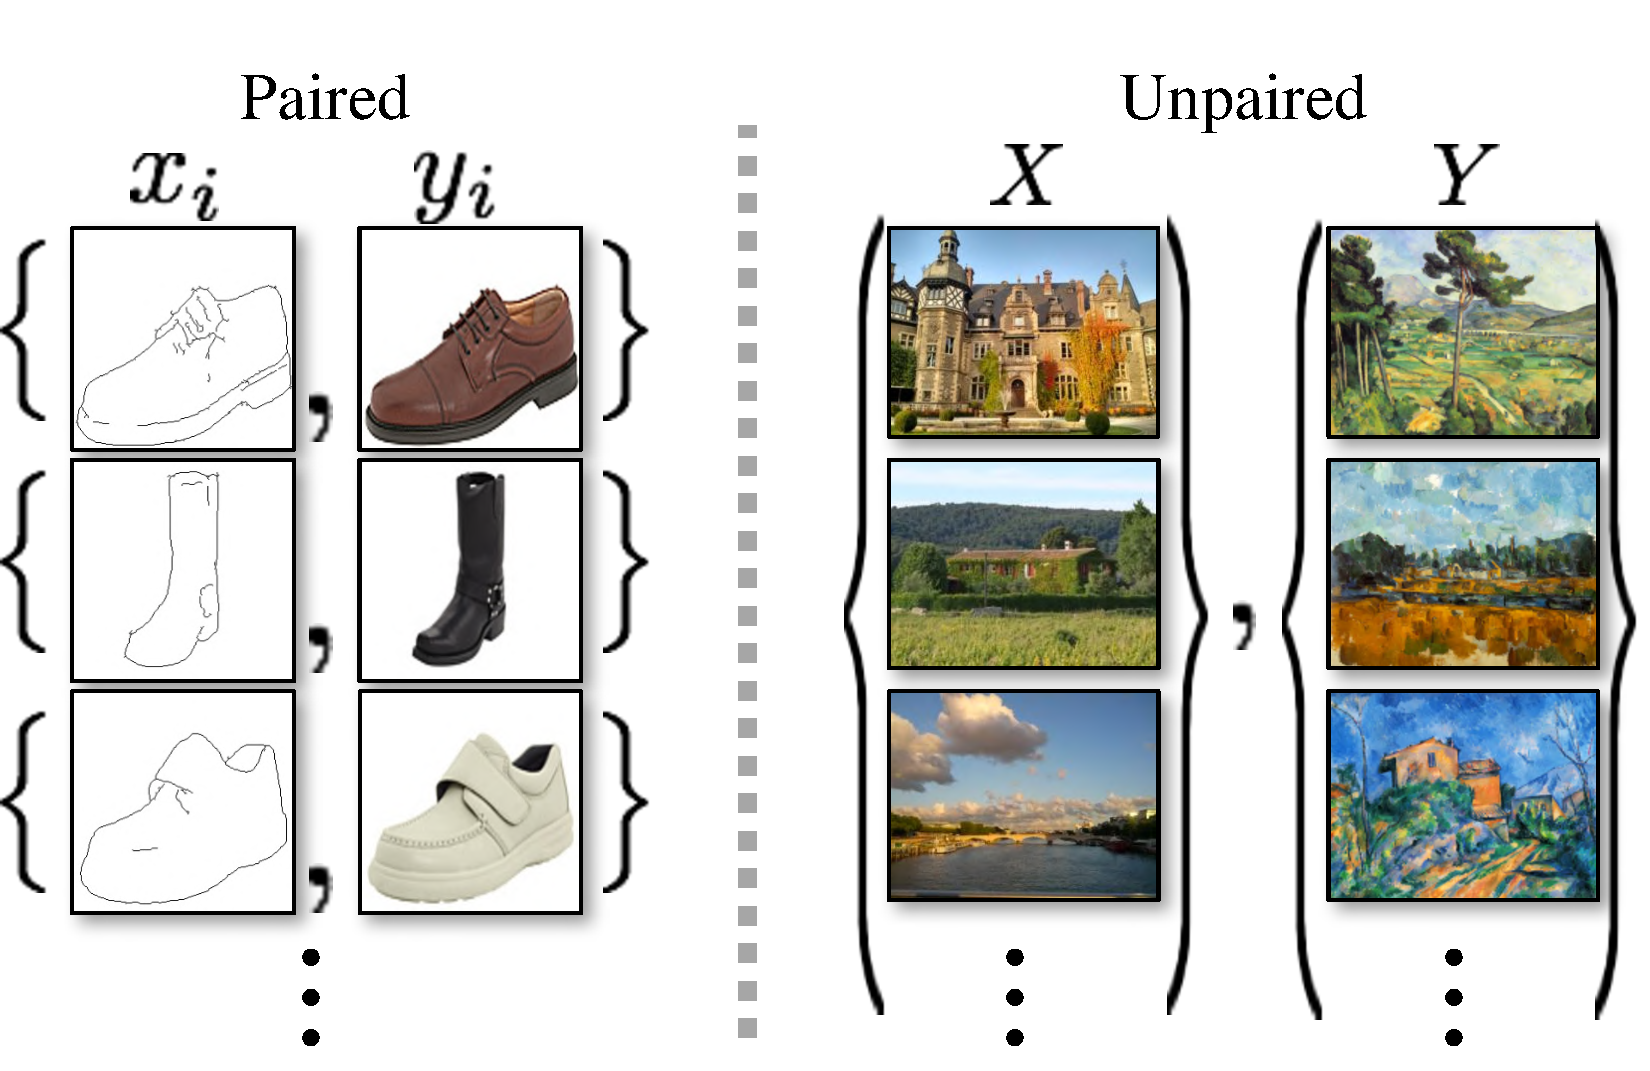
\includegraphics[width=\columnwidth]{src/paired_unpaired2.png}
\caption{\textit{Paired} training data (left) consists of training examples $\{x_i, y_i\}_{i=1}^N$. 
\textit{Unpaired} training data (right) consists of a source set $\{x_i\}_{i=1}^N$ ($x_i \in X$) and a target set $\{y_i\}_{i=1}^N$ ($y_i \in Y$). 
Unpaired training contains no correspondence from the source set $X$ to the target set $Y$. Figure adapted from \cite{zhuUnpairedImagetoImageTranslation2020}.}\label{fig:paired-unpaired}
\end{figure}

Our work uses Cycle-GAN, which is a type of GAN that learns from unpaired training data. Cycle-GAN uses two generators and
two discriminators. A generator $G: X \rightarrow Y$ transforms images from domain $X$ to domain $Y$; a reverse generator
$F: Y \rightarrow X$ transforms images from domain $Y$ to domain $X$. The first discriminator $D_Y$ distinguishes between real images in domain $Y$ and 
generated images from generator $G$; the second discriminator $D_X$ distinguishes between real images in domain $X$ and generated images 
from generator $F$. The Cycle-GAN framework uses a cycle-consistency loss to ensure that the generated images can be transformed back to the original domain.
The cycle-consistency loss is given below, defined by Zhu et al\cite{zhuUnpairedImagetoImageTranslation2020}.
\begin{equation}
\begin{aligned}
\mathcal{L}_{\mathrm{cyc}}(G,F)
&= \mathbb{E}_{x \sim p_{\mathrm{data}}(x)}
\left[\|F(G(x)) - x\|_1\right] \\
&\quad + \mathbb{E}_{y \sim p_{\mathrm{data}}(y)}
\left[\|G(F(y)) - y\|_1\right].
\end{aligned}
\end{equation}

The objective of Cycle-GAN is to minimize the adversarial loss, maximize the discriminator loss, and minimize
the cycle-consistency loss. The key idea for Cycle-GAN is that if an image is transformed from doamin $X$ to domain $Y$ by G, and then it is transformed back to domain $X$ by F, 
the resulting image should be similar to the original image. This cycle-consistency allows the model to not only produces an image that looks like it belongs to the target domain,
but also preserves the content, or the structure of the original image\cite{zhuUnpairedImagetoImageTranslation2020}.

In weather augmentation, cycle-GAN is useful because it generates realistic rainy or foggy images from clear images while it preserves the scene structures and it does not require paired training data. 
However, a limitation of Cycle-GAN, as well as other GANs, is that it is not controllable. It is impossible to control how much wetness, rain, or fog is generated,
and it is impossible to control the depth-dependent effects of rain and fog\cite{zhuUnpairedImagetoImageTranslation2020,tremblayRainRenderingEvaluating2021}. Therefore, our work uses Cycle-GAN to generate rainy and foggy images, but it also uses
a physics-based, depth-aware renderer to generate rain with controllable appearance.


\FloatBarrier

\section{Related Work}

\subsection{Distortion Classification and Evaluation}

Traditional distortion classification models and evaluation use blur indices, noise estimators,
natural scene statistics, image quality metrics, Support Vector Machines (SVM), and K-Nearest
Neighbours (KNN) to evaluate the impact of distortions. Recent distortion classification and
detection models use Convolutional Neural Networks (CNN) and temporal models. Ahn, Kang, and
Sohn train a Y-shaped CNN for joint distortion classification and localization. Other methods
for distortion classification include feature pool, relating metrics with specific distortions,
and Natural Scene Statistics (NSS). The method supports learned distortion features, yet most
datasets focus on controlled distortions rather than natural
weather~\cite{muhammadaliqureshiDistortionClassificationComputer,ahnImageDistortionDetection2017}.


The quality of visual content in images and distortion severity are important factors that
affect performance in high-level tasks, including object classification, object detection, and
scene understanding. Using distortion classification and detection models could help
researchers finetune models that are more resistant to distortions. However, our work helps
finetuning models by presenting a data augmentation framework that increases models’
resilience to rain and fog distortions from training, which does not require distortion
detection and distortion removal process.


\subsection[Current Limitations of Distortion Datasets]{%
Current Limitations of Distortion\\
Datasets}


Current distortion datasets give labels and severity levels, but many examples come from
synthetic, single-type, quality-assessment settings. LIVE, TID2008, TID2013, CSIQ, Waterloo,
KADID-10K, LIVEMD, and MDID help keep a controlled evaluation. However, they do not contain
natural weather withprecise physical labels. Rain, haze, fog, and snow depend on lighting, exposure, particle
density, scene depth, and occlusion. There is a lack of labeled, controlled multi-distortion
datasets. Consequently, classification and localization of multiple distortions remains
challenging due to lack of labeled, controlled
datasets~\cite{muhammadaliqureshiDistortionClassificationComputer,
tremblayRainRenderingEvaluating2021}. Our work adds controlled, artificial distortions, which
addresses lack of labeled, controlled datasets, especially for outdoor datasets.


\subsection{Traditional Rain Rendering}

Garg and Nayar model rain streak photometry and spatio-temporal behavior. Their work links rain
visibility to drop size, velocity, exposure time, scene radiance, camera settings, and drop
shape oscillation. This result matters for rendering because a transparent 2D texture ignores
camera and scene factors. Traditional rain rendering lacks the effect of moisture on the scene,
and it often appears to be unrealistic. For instance, traditional rain rendering lacks wet
surfaces such as water on the ground, and it creates raindrops that are supposed to be hidden
behind buildings~\cite{tremblayRainRenderingEvaluating2021}.
Though, this framework supported rain detection, removal, rendering, and camera-based rain
measurement~\cite{gargVisionRain2007}.


\subsection{Modern Rain Rendering}

Modern rain rendering turns rain models into dataset augmentation for robustness tests. Halder,
Lalonde, and de Charette combine a particle simulator, outdoor illumination estimation, and
rain photometry to render rain and fog over clear driving images. The pipeline preserves labels
from KITTI and Cityscapes while changing weather appearance. Detection and segmentation results
then measure model sensitivity under controlled
rain~\cite{halderPhysicsBasedRenderingImproving2019}.


Tremblay, Halder, de Charette, and Lalonde compare three rendering routes: physics-based,
data-driven, and hybrid. They classify raindrops into rain particles and fog-like rain.
Fog-like rain is a single pixel that contains multiple rain particles; it is located far away from
the camera and appears as fog. The physics-based route combines fog-like rain, rain particles,
and photometric modeling. The renderer estimates outdoor illumination because a raindrop
receives light from a wider angular range (approximately 160 degrees) than the camera's view (70
to 100 degrees). This design improves physical control over a flat overlay. The same design also
depends on sky visibility, environmental symmetry about photometry, and compute
cost~\cite{tremblayRainRenderingEvaluating2021,hold-geoffroyDeepOutdoorIllumination2018,
zhangAllWeatherDeepOutdoor2019}.


The data-driven route uses a GAN-style image translation model. A GAN trains two networks: a
generator synthesizes target-domain images, and a discriminator judges whether each image looks
real or generated. Adversarial training on the generator outputs rainy-looking images. The
output from the generator contains features such as dark sky, rainy environment, wet surfaces
and dim lamination. However, GAN is less controlled, which risks rain density, depth
ordering, and scene consistency. GAN’s focus on global appearance also creates unrealistic
features, such as fake water
reflections~\cite{tremblayRainRenderingEvaluating2021,
isolaImagetoImageTranslationConditional2018,huangMultimodalUnsupervisedImagetoImage2018}.


Tremblay et al. render rain over KITTI, Cityscapes, and nuScenes. They evaluate object
detection, semantic segmentation, and depth estimation under increasing degradation. The paper
reports degrading performances as increasing rain intensity and more robust performances after
finetuning using rain-augmented datasets. The paper reports that outputs from GAN only are
user-rated as the most realistic images; outputs from GAN plus PBR perform the best on data
augmentation~\cite{tremblayRainRenderingEvaluating2021}.


Our work is inspired from the framework from Tremblay et al. our work uses the traditional rain
rendering framework with depth estimation to build rain streaks with controlled,
depth-dependent rain streaks; our work also involves using a Cycle-GAN model that adds rainy
and foggy visual effects.


\subsection{Fog Rendering}

Fog rendering often follows the atmospheric image formation model. Scene radiance attenuates
with distance, while airlight grows along the camera's ray. Sakaridis, Dai, and Van Gool applies
this model to clear Cityscapes images and produce Foggy Cityscapes. Depth makes fog stronger
for far regions rather than uniform across the image. Training with synthetic fog improves
semantic foggy scene understanding, but results depend on depth quality, density choices, and
the synthetic-to-real gap~\cite{sakaridisSemanticFoggyScene2018}.


Clear2Fog extends this direction with monocular depth estimation and atmospheric light
estimation. Monocular depth estimation does not require 3D constructions such as LiDAR; rather,
this paper uses Apple Depth Pro to produce an estimated depth map. The pipeline simulates fog
on clear-weather driving datasets and tries to preserve camera-LiDAR consistency. Without
relying on LiDAR, Clear2Fog remains stable under extreme conditions like fog, snow or haze.
Seeing Through Fog Without Seeing Fog focuses on multimodal perception rather than rendering.
The dataset and fusion model show different failure patterns across camera, LiDAR, radar, and
gated near-infrared
sensors~\cite{mohamedDataEfficiencyStudy2026,bijelicSeeingFogSeeing2020}.


\subsection{Depth Estimation and Application in Distortion Rendering}

Depth provides the geometry needed for natural distortion placement. In haze and fog, depth
sets attenuation and airlight strength. In rain, depth helps determine the severity,
intensity and placement of rain streaks. A renderer without geometry often places
plausible-looking weather in physically inconsistent
locations~\cite{sakaridisSemanticFoggyScene2018,tremblayRainRenderingEvaluating2021}.


Depth estimation models estimate distance from an image or complete sparse sensor depth. The
output supplies an approximate geometry map when a dataset lacks dense ground truth. Jaritz et
al. study sparse and dense depth completion for driving scenes. Depth Anything V2 offers a
modern monocular option trained with synthetic images and pseudo-labeled real images. This
makes Depth Anything V2 useful for RGB-only distortion
rendering~\cite{jaritzSparseDenseData2018,yangDepthAnythingV22024}.


Our work uses the depth-map output from Depth Anything V2 as the guiding parameter for
transparency and appearance of rain streaks and translucency and intensity of fog. The
depth-map output from Depth Anything V2 is stable and reliable, and it is a strong model for
completing our computer vision tasks.


\subsection{Datasets With Distortions}

General distortion and corruption datasets support baselines, but natural weather rendering
requires more geometry and scene context. The distortion survey lists LIVE, TID2008, TID2013,
CSIQ, Waterloo, KADID-10K, LIVEMD, and MDID as major image-quality or multi-distortion
resources. ImageNet-C standardizes common corruption robustness for image classifiers. These
resources help robustness framing. They do not model depth-aware rain, haze, or fog.
\cite{muhammadaliqureshiDistortionClassificationComputer}.


eather-specific datasets match the project more closely. ACDC includes fog, nighttime, rain,
and snow with dense driving-scene annotations and normal-condition correspondences for many
scenes. Foggy Cityscapes and rain-augmented KITTI, Cityscapes, and nuScenes preserve existing
labels while adding synthetic weather. The limitation of these datasets is the lack of
controlled severity or intensity, depth-aware labels, and controlled natural
distortions~\cite{sakaridisACDCAdverseConditions2021,sakaridisSemanticFoggyScene2018,
tremblayRainRenderingEvaluating2021}.


\subsection{BDD100K}

BDD100K serves as a baseline dataset for our work, because the data are large, diverse, and
driving-focused. The dataset contains 100,000 driving videos and supports detection,
segmentation, lane marking, drivable area, and related driving labels. BDD100K also includes
geographic, environmental, and weather variation. The limitation is missing paired
clean/adverse views and controlled severity labels. A depth-aware rain and haze renderer would
turn BDD100K into a controlled robustness testbed while keeping real driving diversity.
\cite{yuBDD100KDiverseDriving2018}.


\nocite{*}
\printbibliography[title={References}]

\end{document}
